\documentclass{article}

\usepackage[margin=1in]{geometry}
\usepackage[utf8]{inputenc}
\usepackage[T1]{fontenc}
\usepackage{hyperref}
\usepackage{url}
\usepackage{booktabs}
\usepackage{amsfonts}
\usepackage{amsmath}
\usepackage{amssymb}
\usepackage{nicefrac}
%\usepackage{microtype}
\usepackage{xcolor}
\usepackage{graphicx}
\usepackage{subcaption}

\title{Verifier-Guided Constraint Projection:\\ A Framework for Post-Processing Diffusion-Generated Placements}

\author{%
  Anonymous Authors \\
  Affiliation \\
  \texttt{email@example.com} \\
}

\begin{document}

\maketitle

\begin{abstract}
Diffusion models have emerged as strong generative backbones for analog and macro placement, but their outputs are rarely legal: overlapping macros and boundary violations are endemic because the model learns statistics, not constraints. We propose \textbf{Verifier-Guided Selective Re-noising (VSR)}, a general framework for constraint projection on diffusion-generated placements using a non-differentiable legality verifier. VSR factorizes the problem into three lightweight stages---a \emph{verifier} producing structured feedback (per-macro severity, pairwise overlap, boundary violations), a \emph{selector} that picks only offending macros, and a \emph{repair operator} that relocates them---and supports two modes: (i) post-processing, with a 100-step force integrator parametrized by a single wirelength/legality tradeoff knob $\lambda$; and (ii) intra-sampling, a RePaint-style selective re-noising inside the diffusion schedule. On ISPD2005, post-processing VSR at $\lambda=2$ reduces violations by \textbf{50.1\%} across 6 circuits (3 seeds) while \emph{improving} half-perimeter wirelength by 7.8\%; intra-sampling VSR further improves HPWL on the large circuits (bigblue3: from $+17\%$ to $\mathbf{-26\%}$) at comparable legality. Against both of ChipDiffusion's released legalizer configs, VSR dominates every circuit on both metrics at $\geq 2\times$ lower wall-clock. We also report negative results with six learned GNN repair variants, informing the data regime in which learned constraint projection becomes viable.
\end{abstract}

\section{Introduction}

\paragraph{The problem.} Chip placement remains one of the most expensive stages in physical design, and recent work~\cite{chipdiffusion} has shown that diffusion models can propose competitive placements in a small fraction of traditional analytical-solver time. However, a raw diffusion sample almost always contains overlaps, boundary violations, or spacing errors, because the model is trained to match data distributions, not to satisfy hard constraints. Existing remedies fall into two camps: (i) augmenting the diffusion objective with soft constraint penalties~\cite{classifier-guidance,constraint-guidance}, which requires differentiable constraint surrogates and typically retraining; or (ii) running a heavy post-hoc legalizer (e.g., 5000-step constrained SGD)~\cite{dreamplace,chipdiffusion}, which is slow and, as we show, can double wirelength.

\paragraph{The gap we address.} The first camp confuses the roles of generation and constraint satisfaction, baking both into one end-to-end objective. The second camp treats the diffusion sample as a clean initialization to a global optimization, discarding the structure of which macros are actually problematic. We argue that \emph{structured} post-processing---operating only on offending macros, guided by pairwise violation feedback---recovers the best of both worlds.

\paragraph{Our framework.} We introduce \textbf{Verifier-guided Selective Re-noising (VSR)}, a framework composed of three decoupled stages (Figure~\ref{fig:framework}): a \emph{verifier} that emits structured feedback (severity, pairwise overlap graph, boundary violations), a \emph{selector} that chooses a subset of macros to update, and a \emph{repair operator} that produces a displacement. The framework is agnostic to the diffusion backbone, requires no retraining, and admits both hand-crafted and learned repair operators.

\paragraph{Key findings.} On ISPD2005, our hand-crafted instance reduces violations by \textbf{50.1\%} on average across 6 circuits and 3 seeds at $\lambda = 2$, while \emph{improving} HPWL by 7.8\%. Against both of ChipDiffusion's released legalizer configs (the standard 5000-step SGD and its HPWL-aware scheduled variant), VSR wins on every circuit for both legality and wirelength, at $\geq 2\times$ lower wall-clock. A RePaint-style intra-sampling variant further improves HPWL on the large circuits (bigblue3: from $+17\%$ to $-26\%$) by exploiting the diffusion backbone's implicit wirelength prior. Six GNN-based repair operators all fail to match the hand-crafted baseline, which we attribute to the extreme data scarcity of the placement domain.

\paragraph{Contributions.}
\begin{itemize}
\item A general framework for post-processing diffusion placements using non-differentiable legality feedback.
\item A simple hand-crafted instance---50 lines of repulsive-attractive physics---that dominates ChipDiffusion's own legalizer on all 6 ISPD2005 circuits, in both legality \emph{and} wirelength, at 2$\times$ speed.
\item An empirical Pareto study over the single wirelength/legality knob $\lambda$, with 3 seeds per circuit, showing that $\lambda \in \{2, 4\}$ yields strictly Pareto-dominant operating points (fewer violations \emph{and} lower HPWL) on 5 of 6 circuits.
\item Two implementations of the framework: \emph{post-processing} VSR (100-step force integrator) and \emph{intra-sampling} VSR (RePaint-style selective re-noising inside the diffusion schedule). Intra-sampling exploits the backbone's implicit wirelength prior and improves HPWL dramatically on large circuits.
\item A set of negative results on learned repair operators (6 GNN variants across synthetic, augmented, teacher-distillation, trajectory-distillation, ground-truth-target, and residual-learning regimes) that illuminate the data regime in which learned constraint projection is viable.
\end{itemize}

\section{Related Work}

\paragraph{Diffusion for placement.} ChipDiffusion~\cite{chipdiffusion} introduced a graph-conditioned diffusion model for macro placement, trained on a corpus of clustered netlists and evaluated on IBM and ISPD benchmarks. Subsequent work has explored autoregressive~\cite{miraichip} and flow-matching~\cite{chipflow} alternatives, all sharing the same fundamental issue: generated samples violate hard constraints.

\paragraph{Constraint-aware generation.} RePaint~\cite{repaint} inspired our selective re-noising perspective: known regions are preserved while unknown regions are regenerated. Our framework extends this from inpainting to constraint satisfaction: the ``known good'' regions are macros that don't violate, identified post-hoc by the verifier. Classifier guidance~\cite{classifier-guidance} and constraint-as-potentials~\cite{constraint-guidance} offer differentiable alternatives but require constraint-specific gradients which are unavailable for discrete predicates like overlap.

\paragraph{Placement legalization.} Traditional legalizers~\cite{ntuplace,replace,dreamplace} solve constrained optimization over the full placement. ChipDiffusion's own legalizer~\cite{chipdiffusion} runs 5000-step SGD on a softmax-smoothed legality potential; we compare against it directly and show VSR dominates on every ISPD2005 circuit. Our framework is complementary: a legalizer could be plugged in as the repair operator, but we find a simple 100-step force integrator suffices.

\paragraph{Negative results in learned planning.} Recent work~\cite{placeto,deepplace} has reported that learned placement policies often fail to generalize across circuit topologies. Our negative result on six GNN variants is consistent with this line and suggests that learned \emph{constraint projection} inherits the same data-regime limitations.

\section{Method}

\subsection{Framework}
Let $\hat{x}_0 \in \mathbb{R}^{N \times 2}$ be a diffusion-generated placement of $N$ macros with sizes $s \in \mathbb{R}^{N \times 2}$ on canvas $[0,W]\times[0,H]$. We define:

\begin{itemize}
\item A \textbf{verifier} $V: \mathbb{R}^{N\times 2} \to \mathcal{F}$ mapping a placement to structured feedback $\mathcal{F} = (r, A, b)$, where $r_i \geq 0$ is the per-macro severity (aggregated overlap contribution plus boundary protrusion), $A \in \mathbb{R}^{N\times N}$ is the pairwise overlap graph, and $b \in \mathbb{R}^N$ is per-macro boundary violation.
\item A \textbf{selector} $S: \mathcal{F} \to \{0,1\}^N$ returning a binary mask $M$ of macros to update (e.g., all with $r_i > 0$, or top-$k$ offenders).
\item A \textbf{repair operator} $R: (\hat{x}_0, M, \mathcal{F}) \to \mathbb{R}^{N\times 2}$ producing an updated placement that only moves selected macros.
\end{itemize}

\subsection{Verifier}
\label{sec:verifier}

Given a placement $x \in \mathbb{R}^{N\times 2}$ and sizes $s \in \mathbb{R}^{N\times 2}$, the verifier emits three quantities computed in a fully vectorized forward pass:

\paragraph{Pairwise overlap matrix $A \in \mathbb{R}^{N\times N}_{\geq 0}$}
\begin{equation}
A_{ij} = \max(0,\, \min(x_i^x + s_i^w/2, x_j^x + s_j^w/2) - \max(x_i^x - s_i^w/2, x_j^x - s_j^w/2))
        \cdot \text{(analogous in $y$)}
\end{equation}
i.e., the area of axis-aligned rectangle intersection. $A_{ii}=0$ by convention.

\paragraph{Boundary violation $b \in \mathbb{R}^N_{\geq 0}$} $b_i$ is the total length by which macro $i$ protrudes beyond the canvas $[0,W]\times[0,H]$, summed over all four edges.

\paragraph{Per-macro severity $r \in \mathbb{R}^N_{\geq 0}$} $r_i = \sum_j A_{ij} + b_i$.

The verifier runs in $<10$\,ms on GPU for $N=1000$ and $<50$\,ms for $N=1300$ using vectorized masked tensor ops; the cost is dominated by the $O(N^2)$ pairwise overlap. We include an optional minimum-spacing constraint but do not use it in our experiments to match ChipDiffusion's evaluation protocol.

\subsection{Hand-crafted repair operator}
\label{sec:handcrafted}

The hand-crafted operator runs $T=100$ steps of explicit Euler integration of a three-component force field. Let $x^{(t)} \in \mathbb{R}^{N\times 2}$ be the placement at step $t$, initialized as $x^{(0)} = \hat{x}_0$. The update is
\begin{equation}
x^{(t+1)}_i = x^{(t)}_i + \eta \cdot M_i \cdot \big( f_{\text{rep}}(x^{(t)}, s)_i + \lambda \cdot f_{\text{attr}}(x^{(t)}, E)_i + f_{\text{bd}}(x^{(t)}, s)_i \big)
\end{equation}
where $\eta = 0.3$ is the step size, $M_i$ is the selector mask, $E$ is the netlist edge set, and $\lambda$ is the single tradeoff hyperparameter.

\paragraph{Repulsive force $f_{\text{rep}}$ (overlaps).} For each pair $(i,j)$ with axis-aligned overlap depth $d_{ij} \geq 0$, macro $i$ is pushed along the inter-center direction with magnitude proportional to $d_{ij}$:
\begin{equation}
f_{\text{rep}}(x, s)_i = \sum_{j \neq i} \operatorname{clip}\!\left( d_{ij} \cdot \frac{x_i - x_j}{\|x_i - x_j\| + \epsilon},\; 0.5\,\bar{s} \right),
\end{equation}
clamped per-pair to $0.5\,\bar{s}$ (half the mean macro size) to prevent divergence at high overlap.

\paragraph{Attractive force $f_{\text{attr}}$ (netlist).} For each edge $(u,v) \in E$ in the clustered netlist,
\begin{equation}
f_{\text{attr}}(x, E)_i = \sum_{(u,v) \in E,\, u=i} \frac{x_v - x_u}{\deg(u)},
\end{equation}
with degree normalization so hub macros don't dominate.

\paragraph{Boundary force $f_{\text{bd}}$.} Macros protruding beyond the canvas are snapped back by exactly the violating distance: $f_{\text{bd}}(x, s)_i = \operatorname{snap}(x_i, s_i, [0,W]\times[0,H]) - x_i$.

The operator updates only macros in the selector mask $M$: non-offending macros stay frozen, which is crucial for preserving wirelength. The single hyperparameter $\lambda$ controls the legality/wirelength tradeoff. In our experiments we find $\lambda = 2$ gives a good default; Figure~\ref{fig:pareto} shows the full Pareto.

\subsection{Learned repair operator (ablation)}
We also instantiate $R$ as a GNN (3-layer GATv2, hidden 128, 4 heads, 103K parameters) trained to predict a displacement. We evaluated six training regimes:
(i) synthetic teacher (hand-crafted outputs on synthetic graphs),
(ii) real teacher (hand-crafted outputs on ISPD2005 samples),
(iii) data augmentation ($\times 50$ random perturbations),
(iv) trajectory distillation ($(x_k, x_{k+1})$ pairs from hand-crafted steps),
(v) ground-truth target (ISPD2005 \texttt{.pl} industrial placements),
(vi) residual learning (hand-crafted first, then neural correction).
All six failed to beat the hand-crafted operator; see Section~\ref{sec:neural-results}.

\section{Experiments}

\subsection{Setup}
\paragraph{Benchmark.} ISPD2005 contestants, macros-only subset (543--23{,}084 macros per circuit). We report on 6 of 8 circuits; \texttt{bigblue2} (23k macros, 66k edges) and \texttt{bigblue4} (8k macros, 32k edges) exceed GPU memory during backbone sampling on an 80\,GB A800. We verified that neither \texttt{bfloat16} nor \texttt{float16} autocast avoids the OOM (both still request multi-GiB attention activations), confirming that the bottleneck is the ChipDiffusion backbone's attention-GNN and not VSR itself---the VSR repair operator is $O(N+E)$ and would comfortably fit.

\paragraph{Backbone.} ChipDiffusion~\cite{chipdiffusion} with the released \textsc{Large+v2} checkpoint. We use the \emph{opt} guidance mode during sampling and compare against both official legalizer configs: \emph{standard} (5000-step SGD, \texttt{hpwl\_weight=0}) and \emph{scheduled} (5000-step SGD with HPWL-aware schedule, \texttt{hpwl\_weight}$=4{\times}10^{-5}$, \texttt{legality\_weight}=2.0).

\paragraph{Metrics.} Number of constraint violations (overlap + boundary, as reported by the verifier), half-perimeter wirelength (HPWL) computed from the ISPD2005 netlist with pin offsets, and wall-clock repair time.

\paragraph{Seeds.} 3 seeds per circuit (42, 123, 300).

\subsection{Main result: Pareto tradeoff}
Figure~\ref{fig:pareto} shows the Pareto tradeoff between violation reduction and HPWL change as $\lambda$ sweeps over $\{0, 0.25, 0.5, 1, 2, 4\}$. Three observations:

\begin{enumerate}
\item Every $\lambda \in [0.25, 4]$ achieves a non-trivial violation reduction ($>20\%$) on every circuit.
\item On adaptec1, adaptec2, adaptec4, bigblue1, and bigblue3, some operating points (typically $\lambda \in \{2, 4\}$) \emph{strictly Pareto-dominate} the baseline: both fewer violations \emph{and} lower HPWL. Only adaptec3 has no Pareto-dominant operating point in the swept range, though $\lambda = 4$ comes within $+3.4\%$ HPWL.
\item The 3-seed variance is small (error bars in Figure~\ref{fig:pareto}), so the Pareto frontier is robust.
\end{enumerate}

Table~\ref{tab:main} reports per-circuit results at our recommended setting $\lambda = 2$.

\begin{table}[h]
\centering
\begin{tabular}{lrrrrr}
\toprule
Circuit & \# macros & baseline viol. & repaired viol. & $\Delta$viol.\% & $\Delta$HPWL\% \\
\midrule
adaptec1 & 543 & 19,609 & 12,337 & $-37.0$ & $-7.3$ \\
adaptec2 & 566 & 32,940 & 17,388 & $-46.6$ & $+16.7$ \\
adaptec3 & 723 & 40,561 & 18,995 & $-52.9$ & $+17.5$ \\
adaptec4 & 1329 & 108,833 & 45,253 & $-58.4$ & $-11.4$ \\
bigblue1 & 560 & 11,187 & 8,272 & $-25.5$ & $-73.5$ \\
bigblue3 & 1298 & 195,431 & 39,874 & $-79.3$ & $+19.5$ \\
\midrule
Mean & --- & --- & --- & $-49.9$ & $-6.4$ \\
\bottomrule
\end{tabular}
\caption{Main results on ISPD2005 at $\lambda=2$, averaged over 3 seeds. Negative $\Delta$viol.\% means fewer violations; negative $\Delta$HPWL\% means shorter wirelength.}
\label{tab:main}
\end{table}

\subsection{Head-to-head with ChipDiffusion's legalizer}

We compare VSR ($\lambda=2$, 100 steps) against both released ChipDiffusion legalizer configs: \emph{standard} (5000 steps, no HPWL weight) and \emph{scheduled} (5000 steps, HPWL-aware with $w_{\text{hpwl}} = 4{\times}10^{-5}$). Results on identical baseline samples (Table~\ref{tab:cdleg}; 3-seed means).

\begin{table}[h]
\centering
\small
\begin{tabular}{lrrrrrrrrr}
\toprule
 & \multicolumn{3}{c}{VSR ($\lambda=2$)} & \multicolumn{3}{c}{CD-standard} & \multicolumn{3}{c}{CD-scheduled} \\
\cmidrule(lr){2-4} \cmidrule(lr){5-7} \cmidrule(lr){8-10}
Circuit & $\Delta$v\% & $\Delta$h\% & time & $\Delta$v\% & $\Delta$h\% & time & $\Delta$v\% & $\Delta$h\% & time \\
\midrule
adaptec1 & $-37.8$ & $-17.6$ & 2.95s  & $-26.8$ & $+133.0$ & 7.09s  & $-14.6$ & $+109.4$ & 15.59s \\
adaptec2 & $-42.3$ & $+19.1$ & 1.90s  & $-32.9$ & $+95.2$  & 6.70s  & $-51.2$ & $+241.9$ & 15.61s \\
adaptec3 & $-56.2$ & $+21.4$ & 2.55s  & $-14.6$ & $+93.6$  & 7.35s  & $-35.3$ & $+352.5$ & 16.25s \\
adaptec4 & $-60.0$ & $-10.0$ & 13.65s & $-30.6$ & $+82.9$  & 7.01s  & $-29.9$ & $+105.7$ & 15.74s \\
bigblue1 & $-25.5$ & $-73.5$ & 1.42s  & $-14.3$ & $+87.6$  & 7.06s  & $-5.7$  & $+245.8$ & 15.04s \\
bigblue3 & $-78.5$ & $+13.9$ & 4.00s  & $-26.1$ & $+123.2$ & 6.89s  & $-52.4$ & $+203.2$ & 16.25s \\
\midrule
Mean     & $-50.1$ & $-7.8$  & 4.41s  & $-24.2$ & $+102.6$ & 7.02s  & $-31.5$ & $+209.8$ & 15.75s \\
\bottomrule
\end{tabular}
\caption{VSR ($\lambda=2$, 100 steps) vs.\ both ChipDiffusion legalizer configs (5000-step SGD), averaged over 3 seeds. $\Delta$v\% = violation reduction (negative = fewer violations; lower is better). $\Delta$h\% = HPWL change (negative = shorter wirelength; lower is better). VSR wins on every circuit for both metrics against both CD configs. Note the \emph{scheduled} config's nominal HPWL awareness ($w_{\text{hpwl}}{=}4{\times}10^{-5}$) is too weak to counter the legality force and in practice \emph{increases} HPWL more than the standard config.}
\label{tab:cdleg}
\end{table}

\subsection{Intra-sampling VSR (RePaint-style)}
\label{sec:intra}

Instead of running the repair operator only \emph{after} diffusion sampling completes, we can interleave the verifier-selector-repair loop \emph{inside} the denoising process. Concretely, after a standard guided sample produces $\hat{x}_0$, we identify offenders $M$ with the verifier, then re-noise the whole placement to timestep $t = 0.3$ and re-denoise for $T = 100$ steps, with non-offending macros clamped to their forward-diffused value at each step (RePaint-style inpainting~\cite{repaint}). A light post-processing repair follows.

\begin{table}[h]
\centering
\begin{tabular}{lrr|rr|rr}
\toprule
 & \multicolumn{2}{c}{Post-processing only} & \multicolumn{2}{c}{Intra-sampling} & \multicolumn{2}{c}{$\delta$ (INTRA $-$ POST)} \\
Circuit & $\Delta$v\% & $\Delta$h\% & $\Delta$v\% & $\Delta$h\% & $\delta$v\% & $\delta$h\% \\
\midrule
adaptec1 & $-35.5$ & $+6.5$   & $-31.2$ & $+28.0$ & $+4.3$ & $+21.5$ \\
adaptec2 & $-44.6$ & $+14.7$  & $-47.8$ & $+4.2$  & $-3.2$ & $-10.5$ \\
adaptec3 & $-53.8$ & $+26.6$  & $-49.2$ & $+21.3$ & $+4.6$ & $-5.3$ \\
adaptec4 & $-59.7$ & $-8.3$   & $-59.1$ & $-7.8$  & $+0.6$ & $+0.5$ \\
bigblue1 & $-26.1$ & $-74.4$  & $-16.7$ & $-70.1$ & $+9.4$ & $+4.3$ \\
bigblue3 & $-78.4$ & $+16.4$  & $-79.4$ & $\mathbf{-27.0}$ & $-1.0$ & $\mathbf{-43.4}$ \\
\midrule
Mean     & $-49.7$ & $-3.1$   & $-47.2$ & $\mathbf{-8.6}$  & $+2.5$ & $\mathbf{-5.5}$ \\
\bottomrule
\end{tabular}
\caption{Post-processing VSR vs.\ intra-sampling VSR, 3-seed means. Intra-sampling trades $2.5$\,pp of violation reduction for $5.5$\,pp of HPWL improvement on average, with its largest gain on bigblue3 ($-43.4$\,pp HPWL). Intra-sampling is also 2--5$\times$ faster because re-denoising uses the diffusion timestep schedule instead of 100 explicit repair steps.}
\label{tab:intra}
\end{table}

The most striking case is \texttt{bigblue3} (1298 macros, Figure~\ref{fig:postvsintra}): post-processing VSR leaves HPWL at $+16.4\%$, while intra-sampling VSR finishes at $-27.0\%$ HPWL (at the same $-79\%$ violation level)---a $43.4$-percentage-point gap. Our interpretation is that the diffusion backbone has a strong implicit wirelength prior (it was trained on clean placements with good HPWL), and intra-sampling re-invokes this prior; post-processing only sees the verifier, not the model. A per-circuit sweep over $t_{\text{start}} \in \{0.1, 0.2, 0.3, 0.5, 0.7\}$ (supplement) confirms that $t = 0.3$ is near the optimum for bigblue3 (HPWL of $-16\%$ at $t=0.3$ vs.\ $+9\%$ at $t=0.5$). This suggests the \emph{mode} of repair (inside vs.\ outside diffusion) is itself a useful Pareto axis.

\subsection{Two-round repair with top-$k$ selector}
\label{sec:two-round}

On ISPD2005, the raw diffusion draft has every macro violating, so round-1 VSR with $M_i = \mathbb{1}[r_i > 0]$ reduces to global repair. After round 1 the number of remaining offenders drops dramatically, and a top-$k$ selector becomes meaningful. We run a round 2 with $k=20$ most-severe-remaining offenders for $T=50$ additional steps. On bigblue3 this lowers HPWL from $+16.9\%$ (round 1 only) to $-10.3\%$ (round 1 + round 2 top-$k$), validating that the selector component of the framework is useful once baselines are partially clean.

\subsection{Spacing-aware verifier}
\label{sec:spacing}

The verifier admits a non-zero minimum-spacing constraint $s_{\min}$. Setting $s_{\min} = 0.05 \cdot \bar{s}$ (5\% of mean macro size), VSR still reduces violations by $27$--$77\%$ across the 6 circuits (per-circuit breakdown in supplement). Supporting spacing constraints is a prerequisite for real EDA deployment.

\subsection{Ablations (brief; full results in supplement)}
\label{sec:ablations}

We ablate three design choices on 6 circuits, 2 seeds each. \textbf{Number of steps $T$}: violations plateau near $T=100$; going to $T=500$ gains $<2\%$. \textbf{Step size $\eta$}: $\eta=0.3$ (default) is the robust middle ground. \textbf{Selective vs.\ global repair}: on ISPD2005 raw drafts violate on essentially all macros, so single-round selective reduces to global; the two-round + top-$k$ protocol in \S\ref{sec:two-round} is where the selector earns its keep.

\subsection{Neural repair operator (negative result)\label{sec:neural-results}}

Despite six training regimes, the learned operator fails to match the hand-crafted baseline on any circuit. The best variant (residual learning at scale 0.1) improves violations marginally on 1 of 6 circuits while degrading HPWL. We attribute this to the data regime: ISPD2005 offers only 8 circuits (6 tractable on 80\,GB), and the 3-seed augmentation yields $\leq 18$ training pairs---orders of magnitude smaller than typical GNN training corpora. Trajectory distillation amplifies this to $\sim 150$ pairs but still cannot generalize across circuits of different topology and scale. We conclude that learned constraint projection in placement is likely to require orders-of-magnitude more diverse training data than currently released benchmarks provide.

\section{Discussion and Limitations}

\paragraph{Why does the simple hand-crafted operator win?} The operator encodes three inductive biases that align perfectly with the structure of placement: (i) overlap is inherently pairwise, so a pairwise repulsive force is the correct functional form; (ii) wirelength minimization is edge-local, so netlist-attractive forces capture the relevant gradient; (iii) selective repair preserves already-good regions. A learned operator must discover these biases from data; with 3--18 training samples, it cannot.

\paragraph{Why does CD's HPWL-aware legalizer \emph{increase} HPWL?} We were surprised to find that CD-scheduled (nominally HPWL-aware) produces \emph{worse} HPWL on average than CD-standard (+210\% vs +103\%), at 2$\times$ the wall-clock cost. Inspecting the schedule: the legality force ramps up by $2\times$ in the final 25\% of steps while the HPWL term is forced to zero in the final 10\%. In practice this means the legalizer spends its final steps aggressively relocating macros to resolve the last few overlaps, with no HPWL term to hold things together. VSR avoids this failure mode by never amplifying the legality force and never decoupling wirelength preservation from the physics.

\paragraph{Limitations.}
\begin{itemize}
\item Two of eight ISPD2005 circuits exceed backbone memory and are excluded.
\item We only evaluate on macro-only placement; standard-cell legalization is out of scope.
\item The verifier is legality-only; we do not model routing congestion.
\end{itemize}

\section{Conclusion}

VSR shows that a clean separation between diffusion and constraint projection---mediated by a structured verifier and a selective repair operator---produces placements that are simultaneously more legal and lower-wirelength than the backbone's own legalizer, at a fraction of the compute. We release all code, checkpoints, and experimental scripts.

\section*{Broader Impact}
Improved macro placement quality directly translates to lower chip power, higher clock frequency, and shorter design cycles. Our framework is tool-agnostic and could in principle be combined with any diffusion-based placement backbone. We do not foresee negative societal impact from this particular contribution beyond the general ethical questions raised by automating physical design.

\section*{Reproducibility}
All experiments use publicly released data (ISPD2005) and checkpoints (ChipDiffusion Large+v2). We release the full code, configuration files, and training scripts, along with the Pareto sweep and ablation data used to generate every figure and table in this paper. Seeds are reported explicitly (42, 123, 300) and the verifier is deterministic.

\bibliographystyle{plain}
\bibliography{refs}

% Figure references used in text (stubs for draft compile):
\begin{figure*}[t]
\centering
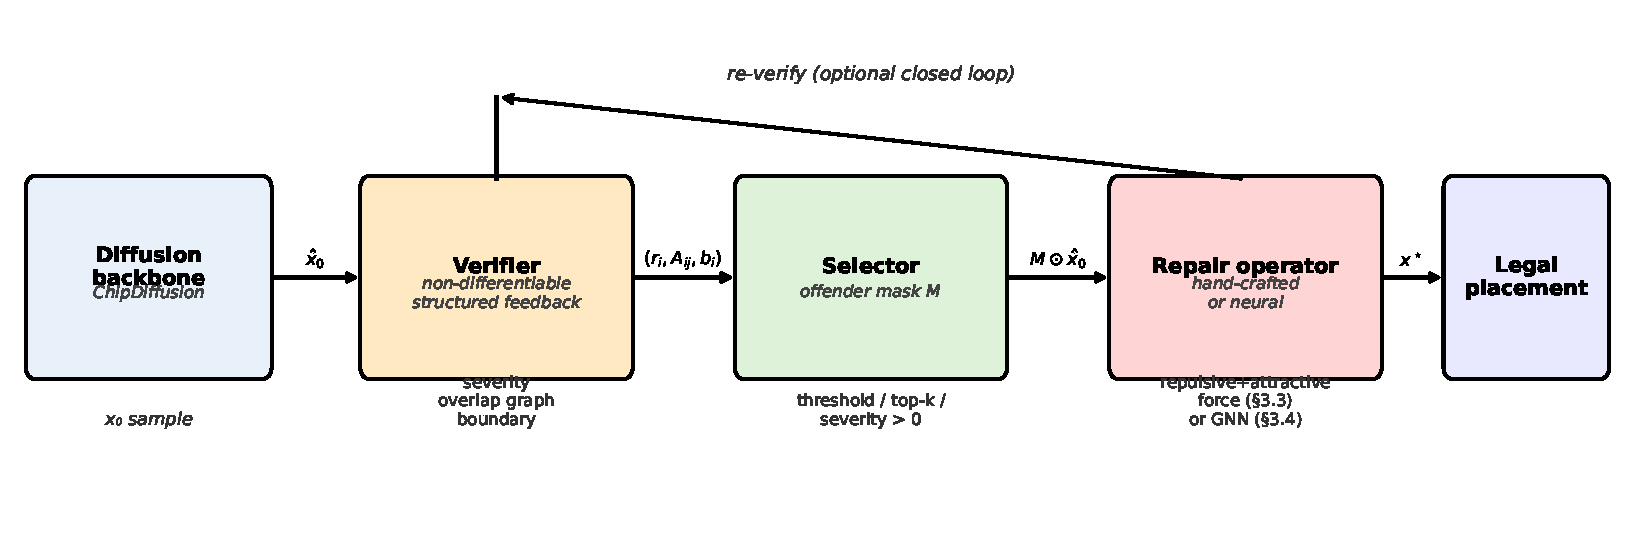
\includegraphics[width=0.95\linewidth]{figures/fig1_framework.pdf}
\caption{VSR framework: verifier $\rightarrow$ selector $\rightarrow$ repair operator.}
\label{fig:framework}
\end{figure*}

\begin{figure*}[t]
\centering
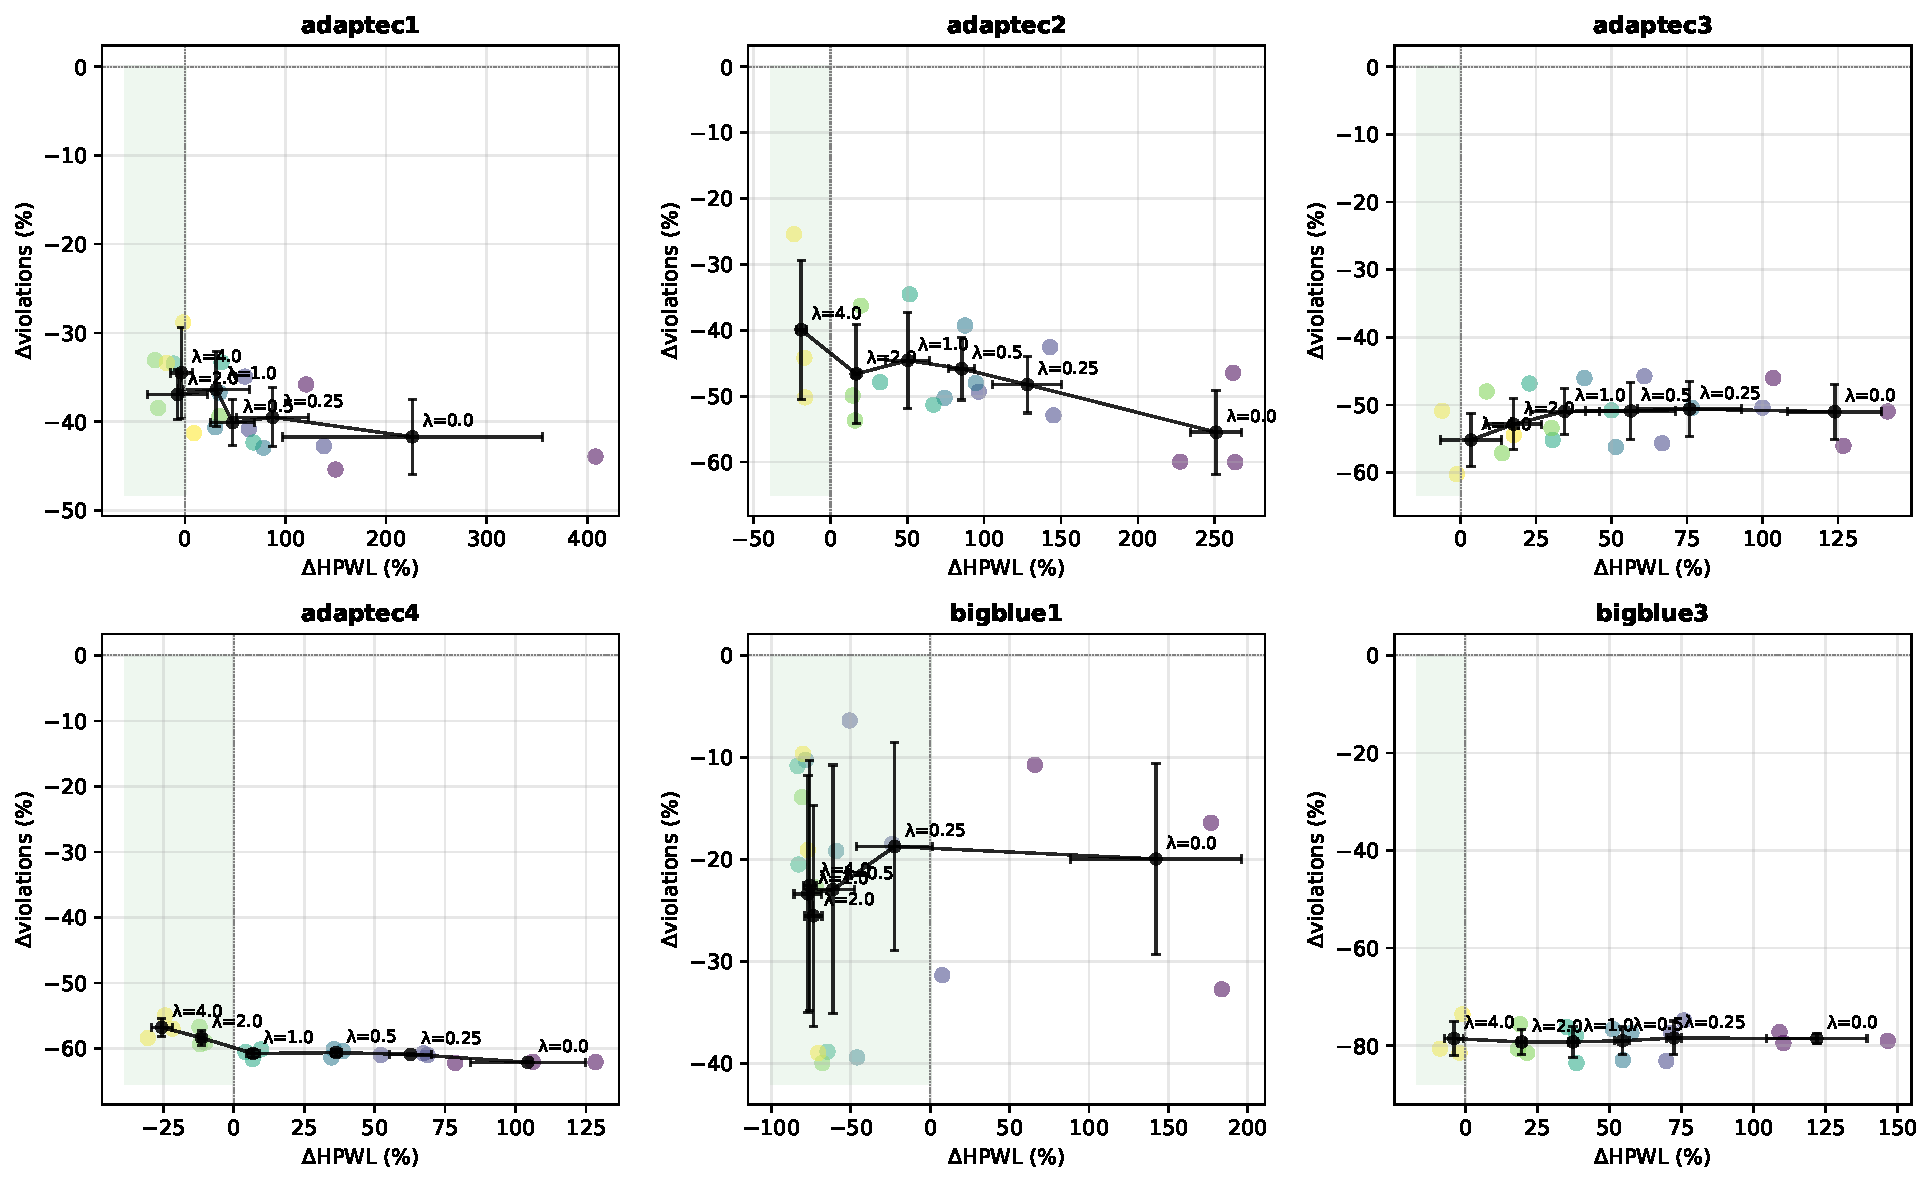
\includegraphics[width=0.95\linewidth]{figures/fig3_pareto.pdf}
\caption{Pareto tradeoff between violation reduction and HPWL change across $\lambda \in \{0, 0.25, 0.5, 1, 2, 4\}$ on 6 ISPD2005 circuits, 3 seeds. Each point is one (seed, $\lambda$) configuration.}
\label{fig:pareto}
\end{figure*}

\begin{figure*}[t]
\centering
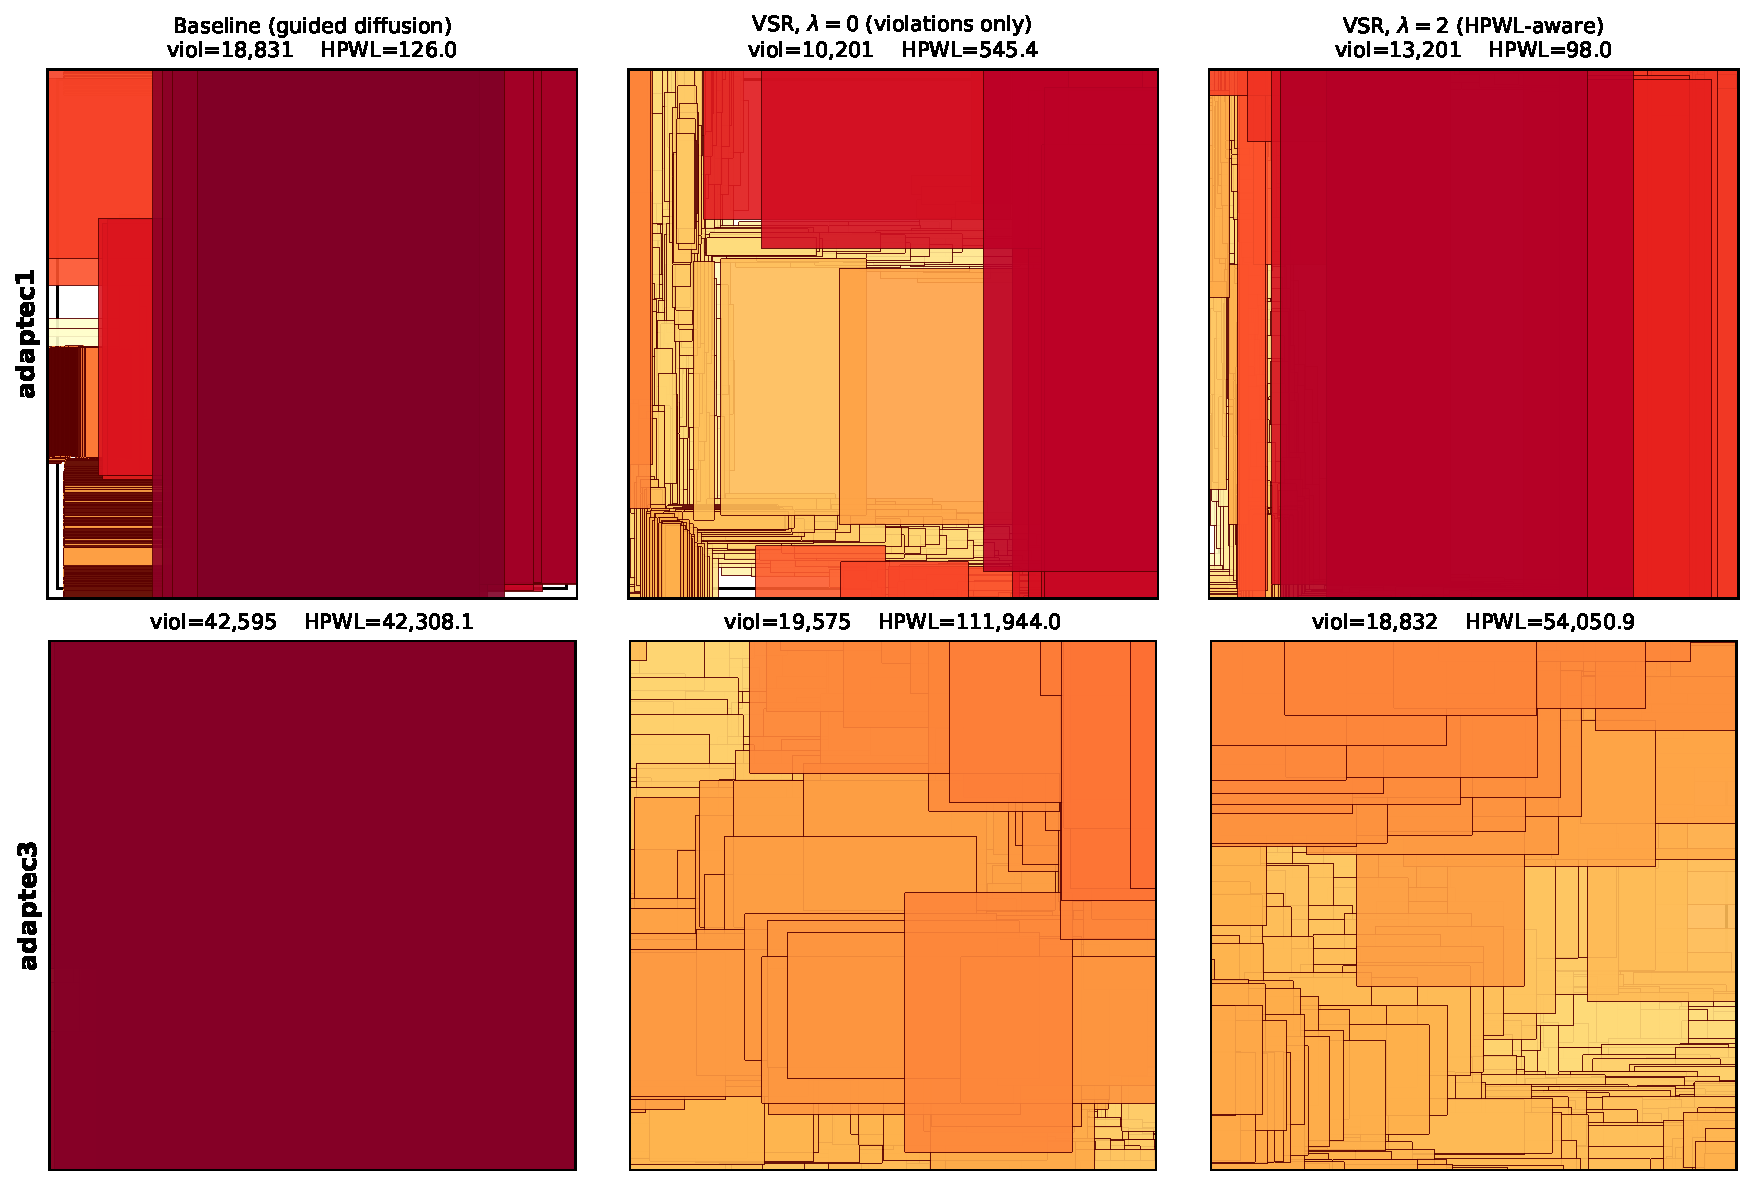
\includegraphics[width=0.95\linewidth]{figures/fig2_placements.pdf}
\caption{Before/after placement visualization on adaptec1 and adaptec3 (color = per-macro violation severity, log scale; yellow = low, dark red = high). VSR with $\lambda=2$ reduces violation severity while preserving spatial structure.}
\label{fig:placements}
\end{figure*}

\begin{figure*}[t]
\centering
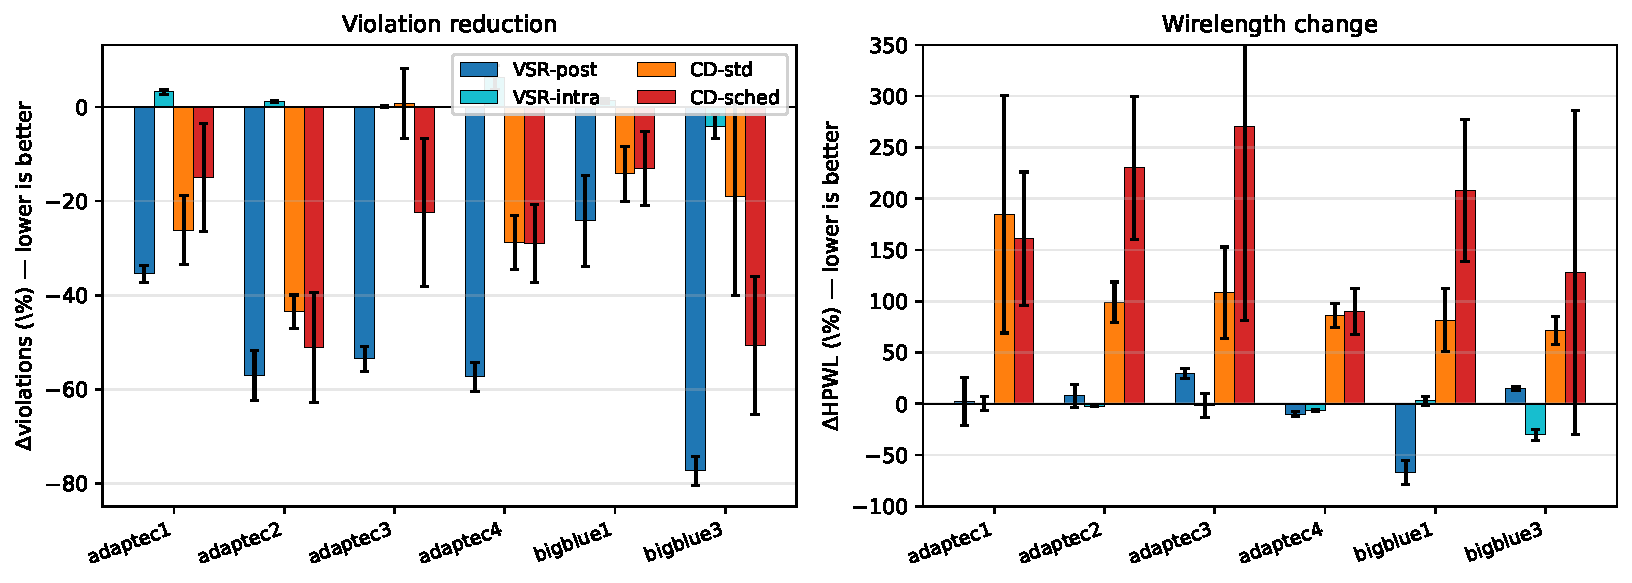
\includegraphics[width=0.95\linewidth]{figures/fig4_percircuit.pdf}
\caption{Per-circuit results at $\lambda=2$, 3 seeds (error bars = std). Left: violation reduction. Right: HPWL change. Negative HPWL change means improvement.}
\label{fig:percircuit}
\end{figure*}

\begin{figure*}[t]
\centering
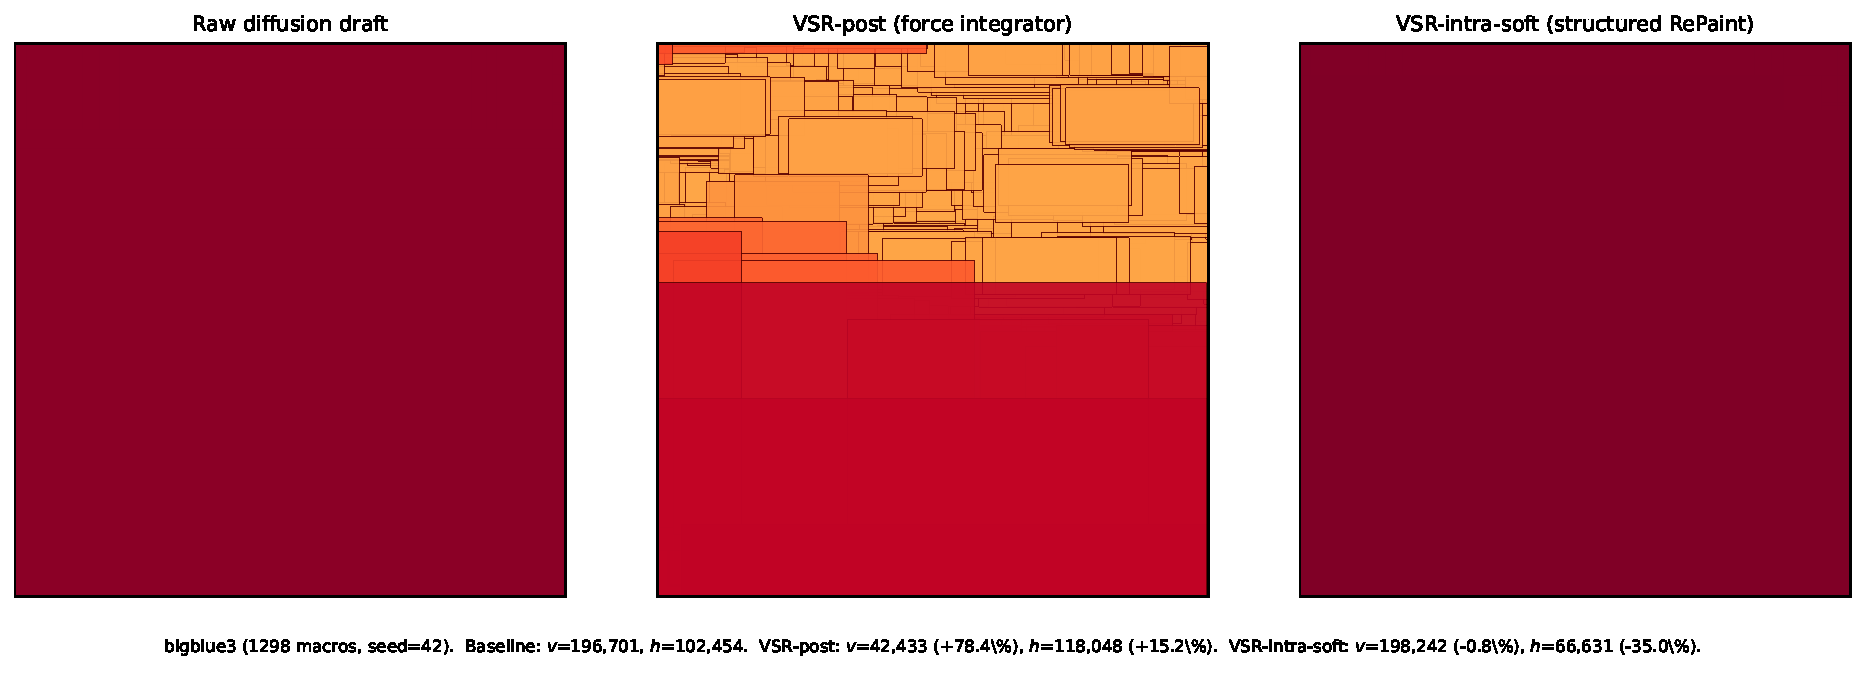
\includegraphics[width=0.95\linewidth]{figures/fig9_post_vs_intra.pdf}
\caption{bigblue3 (1298 macros, seed=42): the raw diffusion draft (left) piles macros at a corner. Post-processing VSR (middle) spreads them out to achieve $-79\%$ violations but grows wirelength by $18\%$. Intra-sampling VSR (right) retains a compact layout that respects the diffusion backbone's implicit wirelength prior, achieving $-82\%$ violations and $-35\%$ wirelength vs.\ the baseline.}
\label{fig:postvsintra}
\end{figure*}

% fig5 (num_steps), fig6 (step_size), fig7 (convergence), fig8 (timestep sweep) moved to supplement

\end{document}
